\documentclass[twocolumn]{article}

\setlength{\columnsep}{30pt}
\usepackage{a4wide,url,changebar}
\usepackage{fancyhdr,xspace}
\usepackage[pdftex]{graphicx}
\usepackage{amsfonts}
\usepackage{amsmath}
\usepackage{amssymb}
\usepackage{fix-cm}
\usepackage{euler}
\usepackage{amssymb}
\usepackage{eso-pic}
\usepackage{helvet}
\usepackage{url}
\pagestyle{fancy}

\usepackage{CJK} 

\newcommand{\inlinegraphic}[2]{
  \dimendef\grafheight=255\dimendef\grafvshift=254
  \grafheight=#1
  \grafvshift=-0.5\grafheight
  \advance\grafvshift by 0.5ex
  \raisebox{\grafvshift}{\includegraphics[height=\grafheight]{#2}\xspace}
}

\fancyhead[L]{\url{theorymine.co.uk}}
\fancyhead[R]{\inlinegraphic{1cm}{images/smalllogo_new.png}}
\fancyfoot[C]{\rm\thepage}



\begin{document}
\begin{CJK}{UTF8}{gbsn}

\renewcommand{\today}{\number\year 年 \number\month 月 \number\day 日}
\renewcommand{\figurename}{图}

\title{
数学定理及其相关简介与说明
}
\author{TheoryMine}

\date{\today}


\newcommand{\nat}{\mathbb{N}}
\newcommand{\bool}{\text{Bool}}
\newcommand{\nl}{\\}

\maketitle

\section*{一 递归与数学归纳法}
\label{recursion}


\begin{figure}[hbt]
% \topline
\begin{center}
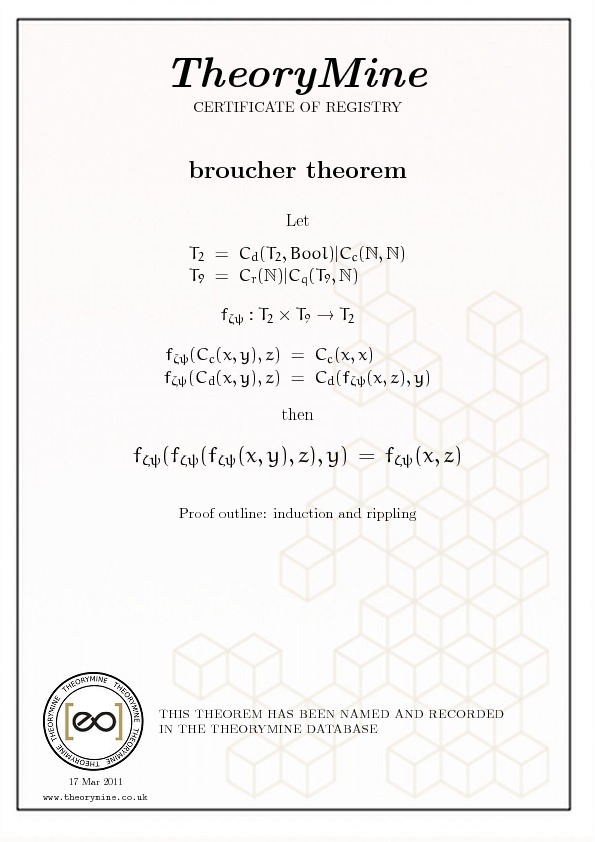
\includegraphics[width=6cm]{certificate_image.jpg}
\end{center}
\caption{Your certificate}
\label{certificate}
% \botline
\end{figure}

\indent \indent  在图\ref{certificate}中您可以预览到您的证书样品。 在本章中我们将对\begin{CJK}{UTF8}{gkai}递归\end{CJK}和\begin{CJK}{UTF8}{gkai}数学归纳法\end{CJK}进行简单的介绍。 这些知识将有助于理解证书中相关的数学的内容的含义。如果您对这些概念已经比较熟悉了,可以跳过本章节,直接参阅\begin{CJK}{UTF8}{gkai}章节\S 二 数学对象\end{CJK}
。\\

%Your certificate is given in Figure .  In order to understand 
%it, it is first necessary to understand the concepts of {\em recursion} and {\em
%  induction}.  In this section we provide an elementary introduction to these
%concepts for those not already familiar with them.  Those who do not need this
%introduction can proceed to \S

\indent \indent 所有新产生的数学对象(详见\begin{CJK}{UTF8}{gkai}章节\S 二 数学对象\end{CJK})和新定义的数学函数(详见\begin{CJK}{UTF8}{gkai}章节\S 三 数学函数\end{CJK})都是通过递归定义的方式生成的。该定义法的特点是:定义式中包含被定义对象作为参数。而这些通过递归来定义的数学对象和数学函数,常用数学归纳法来证明。这些定义方式和证明方法咋一听来似乎有点费解,有点死循环的感觉。 然而当您了解了其中规律以后,就会觉得他们是多么的简练。\\

%Both new mathematical objects (see \S\ref{objects}) and new defined functions
%(see \S\ref{functions}) are defined using recursion. This is a form of
%definition in which the body of the definition contains the thing being
%defined. This sounds circular, but it need not be. Similarly, theorems about
%recursive objects and functions are usually proved by mathematical induction. At
%first sight, this form of proof can also appear to be circular, but it is not
%once you understand it.

\subsection*{1.1 自然数}
\label{naturals}

\indent \indent \indent 如下我们所熟悉的\begin{CJK}{UTF8}{gkai}自然数\end{CJK},采用了递归的方法来定义,例如:非负的整数$0, 1, 2, 3, \ldots$ 。
%Consider, the following recursive definition of the, so called, {\em natural
%  numbers}, i.e., the non-negative whole numbers $0, 1, 2, 3, \ldots$.
\begin{eqnarray}
 \nat & = & 0 |
Suc(\nat) \label{nats}
\end{eqnarray}

\indent \indent 其中,$Suc$ 被称为\begin{CJK}{UTF8}{gkai}后继函数(successor function)\end{CJK}。 该定义采用Backus-Naur Form\footnote{\url{http://en.wikipedia.org/wiki/Backus_Naur_Form}} {\sc
  bnf})的格式。 自然数集合$\nat$被以上式子所定义。等号左边定义是被定义对象,等号右边是定义表达式。该表达式被符号$|$分为两个部分。任意一个自然数都可以被该定义式定义到。值得注意的是自然数集合$\nat$,即被定义对象,出现在表达式的第二个部分$Suc(\nat)$内。该部分被称为\begin{CJK}{UTF8}{gkai}(step case)\end{CJK};第一部分被称为\begin{CJK}{UTF8}{gkai}(base case)\end{CJK}。\\
  
%where $Suc$ is called the $successor$ $function$. This definition is in Backus-Naur
%Form\footnote{\url{http://en.wikipedia.org/wiki/Backus_Naur_Form}} ({\sc
%  bnf}). $\nat$, the set of natural numbers, which is being defined, is to the left
%of the $=$ sign. On the right of the $=$ sign is the body of the
%definition. This consists of two cases, separated by a vertical line $|$. Any
%particular natural number corresponds to one of these cases.  Note that $\nat$
%occurs in the second case $Suc(\nat)$. This is a {\em step case}. The other case,
%$0$, is a {\em base case}.

\indent \indent 被定义对象出现在自身的定义表达式中就是一种\begin{CJK}{UTF8}{gkai}递归定义\end{CJK}的明显的特征。把这种定义方式联想成螺旋模型而不是圆型模型,就好理解很多了。 $0$就是这个螺旋的中心点,每一个$Suc$的结果都形成一个完整的环。 这种流程就能生成自然数集合的定义式$0, Suc(0), Suc(Suc(0)), Suc(Suc(Suc(0))), \ldots$。 其中每次调用$Suc$都使得结果加1。这种表达方式可追溯到数学家Giuseppe Peano\footnote{\url{http://en.wikipedia.org/wiki/Peano_axioms}} (1858-1932)。\\

%The occurrence of a concept in the body of its own definition is an indication
%that the definition is {\em recursive}. Think of this recursive definition, not
%as a circle, but as a spiral.  $0$ is at the centre of the spiral; each
%application of $Suc$ winds the spiral out by a complete circuit.  This process
%generates a representation of the natural numbers of the form $0, Suc(0), Suc(Suc(0)),
%Suc(Suc(Suc(0))), \ldots$, where each application of $Suc$ increases the number by
%1. This representation is due to the mathematician Giuseppe
%Peano\footnote{\url{http://en.wikipedia.org/wiki/Peano_axioms}} (1858-1932).

\indent \indent 由于$0$和$Suc$被用于新的数学对象的类型,它们称为\begin{CJK}{UTF8}{gkai}构造函数\end{CJK}。值得注意的是,我们故意没有定义它们本身。因为作为基础的数学对象,它们被用于定义其他的数学对象和函数。这种递归定义式优势需要在某个点停止展开,这个点就和构造函数相关。\\
%$0$ and $Suc$ are called {\em constructor functions}, because they are used to
%%{\em deliberately} not defined. They are taken as primitive mathematical objects
%and are used in the definitions of other mathematical objects and defined
%functions. Definitions have to stop unfolding at some point, and that point is
%with the constructor functions.

\indent \indent 布尔值$true$和$false$可以通过退化形式的的递归来定义。 该定义式由两个基础范例(base case)组成且没有进阶范例(step case): $Bool = true | false$。\\

%The boolean truth values, $true$ and $false$, can be
%defined by a degenerate form of recursion, in which there are two base
%cases and no step cases: $Bool = true | false$.

\indent \indent 我们将用$Bool$ 和 $\nat$来作为通过递归来定义新的数学对象的基础,正如在\begin{CJK}{UTF8}{gkai}章节数学对象\end{CJK}将介绍的。他们将出现在一些构造函数的定义式中。\\
%We will use $Bool$ and $\nat$ as the basis for defining new sets of recursively
%defined mathematical objects, such as those explained in \S\ref{objects}
%below. They will occur as some of the inputs to constructor functions.

\subsection*{1.2 加法函数}
\label{addition}

\indent \indent \indent 加法函数$+$可以通过递归的形式来定义。 它接受两个$nat$类型的数作为参数并返回一个同类型的值。类似的,该定义有一个基础范例(base case) 和一个进阶范例(step case)。
%The function $+$ can also be defined recursively. It takes
%two members of $\nat$ as inputs and returns one as output.  It
%also has a base case and a step case.

\begin{eqnarray}
 + & : & \nat \times \nat \rightarrow \nat \label{type} \\
0+y & = & y  \label{base} \\
Suc(x)+y & = & Suc(x+y) \label{step}
\end{eqnarray}

\indent \indent 第(\ref{type}) 行的意思是 + 接受两个自然数作为输入并返回一个自然数作为输出。第(\ref{base})行和第(\ref{step}) 行一起构成了+的递归定义。在等号(=)左边的表达式被称为定义式的
\begin{CJK}{UTF8}{gkai}头部(head)\end{CJK},在等号(=)右边的被称为定义式的\begin{CJK}{UTF8}{gkai}主体(body)\end{CJK}。第(\ref{base})行是一个基础范例,在该情况下+并不出现在等号右边的定义式中。第(\ref{step})行是一个进阶范例,该情况下+出现在等号右边的定义式中。递归发生在+的第一个参数$x$上。该$x$被称为\begin{CJK}{UTF8}{gkai}递归变量\end{CJK}。值得注意的是,针对自然数$\nat$定义得每一项都有一个相对的表达式定义在加法操作中。这些表达式中的X仅能被实例化为一项自然数的定义,比如$0$ 和 $Suc(x)$。由于这种定义方法,在递归变量上体现出和数学对象的类型结构范围的直接关联关系,因此该类型的递归定义被称为\begin{CJK}{UTF8}{gkai}结构化(structural)\end{CJK}。\\

%Line (\ref{type}) says that + takes two natural numbers as inputs and
%outputs one natural number. Lines (\ref{base}) and (\ref{step}) constitute the
%recursive definition of +. The formulae to the left of the = sign are the {\em heads}
%of the definition and those to the right are the {\em body}.  Line (\ref{base})
%is a base case, in which + does not occur on the right hand side. Line
%(\ref{step}) is a step case, in which + {\em does} occur on the right hand side.
%The recursion is on $x$, the first input of +.  $x$ is called the {\em recursion
% variable}.  Note that for each of the two cases in the definition of $\nat$ there
%is one equation in the definition of +. Moreover, in each of these equations $x$
%is instantiated to exactly one of the cases in the definition of $\nat$, i.e., $0$
%and $Suc(x)$. This kind of recursive definition is called {\em structural}, as it
%directly corresponds to the structure of the type of objects that its recursion
%variable ranges over.


\indent \indent 在加法函数的进阶范例的定义中,出现了加法符号(+),这种自定义的方式并不会引起死循环定义。类似的,这种定义方式可以被理解成螺旋状定义。而这次递归螺旋的方向是向内的。从一个任意的值$x$开始,比如$Suc(0)$,进阶范例就成为$Suc(Suc(0)) + y$。首先将其转化成$Suc(Suc(0) + y)$, 然后再转化成$Suc(Suc(0 + y))$。现在基础范例就可以被写成$Suc(Suc(y))$,然后结果就可以被计算出来。请注意在进阶范例的的特殊的组织方式:相对于头部表达式中的$x$, 主体表达式中的$x$被逐步转换成更小的值的范围的定义方式。$\nat$的定义方式是{\em well founded},该属性保证了该类型的成员的值不能无限减小,任意的值在减少后最终会终止于$0$。这确保了加法函数的演算重重能够终止。即,进阶范例的使用次数是有穷的,最终基础范例将可被应用,此时演算结束。为了将区别出这种函数(如示例中加法函数,定义中带有构造函数($0$和$Suc$) ),他们被称为\begin{CJK}{UTF8}{gkai}已定义函数\end{CJK}。

%The occurrence of + in the body of the step case does not make the definition
%circular. Again, it can be seen as a spiral definition. This time the recursion
%spirals inwards. Starting with some particular value of $x$, say $Suc(Suc(o))$, the
%step case is applied to rewrite $Suc(Suc(0))+y$ first to $Suc(Suc(0)+y)$ and then to
%$Suc(Suc(0+y))$. Now the base case of the definition can be used to rewrite this as
%$Suc(Suc(y))$ and the calculation is finished. Notice how the step case is organised
%so that + is applied to a smaller occurrence of $x$ in the body of the
%definition than in the head. $\nat$ has been defined to be {\em well founded},
%which means that a sequence of its members cannot keep getting smaller forever:
%sooner or later it will reach 0. This means that any calculation carried out
%using + will eventually stop. We can only apply the step case a finite number of
%times. Eventually, only the base case will be applicable and, after the base
%case, nothing will be applicable. To contrast functions such as + with the
%constructor functions, such as 0 and $Suc$, + is called a {\em defined function}.

\subsection*{1.3 数学加法结合律及其归纳法证明}
\label{assoc-proof}

\indent \indent \indent 加法函数具有\begin{CJK}{UTF8}{gkai}结合律\end{CJK}的属性。比如,如果你要对三个数求和,进行加法运算的次序是无关紧要的,先对前两个数求和先对后两个数求和的结果是一样的。这种性质可以用如下数学公理表达:

%The function + is {\em associative}, i.e., if you add three numbers, it doesn't
%matter if you add the first to the sum of the other two or the sum of the first
%two to the third --- you'll get the same answer. This fact can be formalised as
%the theorem:
\begin{eqnarray}
 u+(v+w) & = & (u+v)+w \label{assoc}
\end{eqnarray}
而如上的数学公理可以用\begin{CJK}{UTF8}{gkai}数学归纳法\end{CJK}证明。\\
%which can be proved by {\em induction.}

\indent \indent数学归纳法和递归有着紧密的联系。由递归方法定义的 数学函数所构成的数学定理,应用到同样由递归方式定义的数学对象时候, 比如具有结合律性质的加法,通常使用数学归纳法来证明。首先从要证明的数学定理中选取一个变量作为\begin{CJK}{UTF8}{gkai}归纳变量(induction variable)\end{CJK}。在这个例子中,我们选择 \footnote{见如下文章来查看选择 $v$ 或者 $w$的效果} $u$,该变量同事出现在等式的左边和右边。\\

\indent \indent 和递归定义一样,一个归纳证明也分为基础范例和进阶范例两部分。

%Induction is closely related to recursion. Theorems composed of recursively
%defined functions applied to recursively defined objects, such as the
%associativity of +, are usually proved by induction.  Firstly, an {\em induction
% variable} is chosen from those variables in the theorem.  In this case we will
%choose \footnote{See below for the effect of choosing $v$ or $w$} $u$, which is
%the first variable on each side of the theorem.

%Just like a recursive definition, an inductive proof is divided into base and
%step cases.
\begin{itemize}
\item 在基础范例的情况下,通过分别实例化归纳变量成为数学对象定义中基础范例理的值,来证明该公理成立。在我们的例子中,只有一个基础范例,即$u$被实例化为$0$。因此我们需要证明如下特定的数学公理:
%\item In the base cases, the theorem is proved with the induction variable being
%  instantiated to each of the base cases of the mathematical objects it ranges over. In
%  our case, there is only one base case, in which $u$ is instantiated to
%  $0$. So, we have to prove the special case of the theorem:
\begin{eqnarray*}
 0+(v+w) & = & (0+v)+w
\end{eqnarray*}
\item 在进阶范例情况下,首先假设归纳变量对于该公理是成立的。这被称为\begin{CJK}{UTF8}{gkai}归纳假设\end{CJK}。接着我们把归纳变量实例化成数学对象的定义中的后继的值,这时该表达式称为\begin{CJK}{UTF8}{gkai}归纳结论\end{CJK}。通过证明归纳结论来证明进阶范例情况下的定理。在证明过程中,归纳假设可以作为已知的条件来使用。这种类型的归纳法被称为\begin{CJK}{UTF8}{gkai}结构化(structural)\end{CJK},因为证明过程中的范例重的归纳变量的范围和数学对象的定义的结构紧密的联系在一起。
\end{itemize}
%\item In the step cases, the theorem is assumed to hold for the induction
%  variable. This is called the {\em induction hypothesis}. The theorem is then
%  proved with the induction variable being instantiated to each of the step cases of the
%  mathematical objects it ranges over. These are called the {\em induction
%    conclusions}. During the proof of an induction conclusion, we are allowed to
%  use the induction hypothesis. This kind of induction is called {\em
%    structural} because its cases correspond to the structure of the type of
%  objects that its induction variable ranges over.

\indent \indent 在我们的例子中只需要证明一个进阶范例。在该归纳结论中,$u$被实例化为$Suc(u)$。于是我们有如下归纳假设:
%  In our case, there is only one step case. In its induction conclusion, $u$ is
%  instantiated to $Suc(u)$. So, we assume the induction hypothesis:
\begin{eqnarray}
 u+(v+w) & = & (u+v)+w \label{ih}
\end{eqnarray}
%and then have to prove the induction conclusion:
然后我们所需要证明的归纳结论如下所示:
\begin{eqnarray*}
 Suc(u)+(v+w) & = & (Suc(u)+v)+w
\end{eqnarray*}

\indent \indent 初看之下该归纳证明是种死循环逻辑。在证明进阶范例是我们已经\begin{CJK}{UTF8}{gkai}假设了该数学定理是成立的\end{CJK}。实际上该归纳证明也是一个螺旋式的流程。我们从证明螺旋该数学定理的中心点(基础范例)成立为出发点,接着顺着进阶范例来证明对于螺旋的第一圈是成立的,再接着接着第二圈,第三圈直到第任意圈上。\\

% At first sight, inductive proofs look circular. During the proof of the step
%case, we {\em assume the theorem already holds}. But, once again, the
%inductive proof is really spiral. We start by proving that the theorem holds for
%the centre of the spiral (the base case), then the step case can be used to
%prove that it holds for one circuit of the spiral, then for two circuits, then
%three, and so on for any number of circuits.

\indent \indent \begin{CJK}{UTF8}{gkai}基础范例\end{CJK}可以应用两次加法的递归定义中的基础定义,$0+y=y$。利用该转换公式,左边的表达式可以在两步内转化成右边的表达式,过程如下所示:
%{\bf The base case} can be proved by two applications of the
%  base case of the recursive definition of +, $0+y=y$. These can be used to
%  rewrite the left-hand side of the base case into the right-hand side in two
%  stages, as follows:
\begin{center}
$\begin{array}{rcll}
0+(v+w) & = & v+w     & $by (\ref{base})$ \\
        & = & (0+v)+w & $by (\ref{base})$ \\
\end{array}$
\end{center}
至此,基础案例已被证明。
%At this point the base case is proved.

\indent \indent 在\begin{CJK}{UTF8}{gkai}进阶范例\end{CJK}中,归纳结论可以通过运用三次加法递归定义中的进阶定义($Suc(x)+y = Suc(x+y)$ )和一次归纳假设来完成证明。 等号左边的表达式在通过4步的转换后可被变化成等号右边的表达式,具体信息如下:
%In {\bf the step case}, the induction conclusion can be proved by three
%applications of the step case of the recursive definition of +, namely $Suc(x)+y =
%Suc(x+y)$ and an application of the induction hypothesis.  The left-hand side of
%the induction conclusion is rewritten the right-hand side in four stages, as
%follows:
\begin{center}
$\begin{array}{rcll}
Suc(u)+(v+w) \\
            &= & Suc(u+(v+w)) & $by (\ref{step})$ \\
           & = & Suc((u+v)+w) & $by (\ref{ih})$ \\
           & = & Suc(u+v)+w   & $by (\ref{step})$ \\
           & = & (Suc(u)+v)+w & $by (\ref{step})$ \\
\end{array}$
\end{center}
至此,进阶范例已被证明,且整个加法结合律的归纳证明也完整了。\\
%At which point the step case is proved. This completes the inductive proof of
%the associativity of +.

\indent \indent 有时,证明过程中不仅仅需要递归定义和归纳假设。可能会需要到之前已被证明的数学定理的支持,比如已被之前顾客购买的某定理。当一个数学定理已这种中间形式被使用时,被称为\begin{CJK}{UTF8}{gkai}引理\end{CJK}。\\
%Sometimes, a proof requires more than just the recursive definitions of the
%defined functions and the induction hypothesis. It is necessary also to use
%previously proved theorems, perhaps purchased by another customer. When used in
%this way, theorems are often called {\em lemmas}.

\indent \indent 为了进一步说明引理的在证明中的使用,我们再证明一次加法的结合律,不过这次我们选择$v$为归纳变量。此时,证明过程重需要如下两个引理:
%To illustrate the use of lemmas in a proof, consider again the proof of the
%associativity of +, but this time using induction on $v$. This version of the
%proof requires the following two lemmas:
\begin{eqnarray}
 x+0 & = & x  \label{cbase} \\
x+Suc(y) & = & Suc(x+y) \label{cstep}
\end{eqnarray}
本质上,他们是加法定义中(\ref{base})和(\ref{step})的转换形式。此时基础范例的证明如下:
%which are commuted versions of the defining equations of +: (\ref{base}) and
%(\ref{step}). This time the proof of the base case is:
\begin{center}
$\begin{array}{rcll}
u+(0+w) & = & u+w     & $by (\ref{base})$ \\
        & = & (u+0)+w & $by (\ref{cbase})$ \\
\end{array}$
\end{center}
进阶范例的证明如下:
%and that of the step case is:
\begin{center}
$\begin{array}{rcll}
u+(Suc(v)+w) & = & u+Suc(v+w)   & $by (\ref{step})$ \\
           & = & Suc(u+(v+w)) & $by (\ref{cstep})$ \\
           & = & Suc((u+v)+w) & $by (\ref{ih})$ \\
           & = & (Suc(u+v))+w & $by (\ref{step})$ \\
           & = & (u+Suc(v))+w & $by (\ref{cstep})$ \\
\end{array}$
\end{center}
请注意证明过程中同时需要加法的递归定义和引理。如果我们选用$w$作为归纳变量又是什么结果呢?
%Notice how both the defining equations and the lemmas are required. What is
%needed for the proof by induction on $w$?


\section*{二 数学对象}
\label{objects}

\begin{eqnarray*}
*********DATA TYPE1*********
\end{eqnarray*}

\indent \indent 证书的该部分包含了\begin{CJK}{UTF8}{gkai}新\end{CJK}的数学对象集合的定义。 请参阅在\begin{CJK}{UTF8}{gkai}章节\S\ref{naturals} 1.1 自然数\end{CJK}关于自然数的递归定义公式 (\ref{nats})。\\

%This part of the certificate contains the definitions of one or more {\em new}
%sets of mathematical object. Compare them with formula (\ref{nats}), the
%recursive definition of the natural numbers, in \S\ref{naturals}.

\indent \indent 等号左边的是被定义的新的数学对象集合的名字。在TheoryMine里,通常限制这些新的数学对象的名字为$T$,或 $T_n$ 如果是相对与某些数$n$。等号右边的定义的主体部分,该部分被 $|$ 符号分割成不同的范例。每个范例都由一个构造函数组成,该函数可以有零到多个参数。构造函数的参数可以是$Bool$, $\nat$和之前被定义的或在本证明书中被定义的集合。在最后一个被定义的范例理,通过构造函数来定义进阶范例,或是基础范例。正如\begin{CJK}{UTF8}{gkai}章节\S\ref{naturals}1.1 自然数\end{CJK}中的 $0$,$Suc$,$true$ 和 $false$一样,构造函数作为一种数学定义的原始成分而不被定义。

%To the left of the = signs are the names of the new sets of mathematical objects
%being defined.  The TheoryMine naming convention for these new sets of objects
%restricts their names to $T$ or $T_n$ for some number $n$. To the right of the =
%signs are the bodies of these definitions expressed as a number of cases
%separated by the $|$ symbol. Each case consists of a new constructor function
%with zero or more inputs. The TheoryMine naming convention for these new
%constructor functions restricts their names to $C_l$ for some letter $l$. The
%inputs to these constructor functions can be $Bool$, $\nat$, the names of previously
%defined sets of objects and the name of the set being defined. In this last
%case, the constructor functions will define step cases, otherwise, they will
%define base cases. Just as with $0$, $Suc$, $true$ and $false$ in
%\S\ref{naturals}, these new constructor functions are primitives that are not
%themselves defined.


\section*{三 数学函数}
\label{functions}

\begin{eqnarray*}
*********DATA TYPE2*********
\end{eqnarray*}

\begin{eqnarray*}
*********THEORY*********
\end{eqnarray*}

\indent \indent 证书的该部分包含了一个或者多个数学函数的定义。与之相对的是\begin{CJK}{UTF8}{gkai}章节\S\ref{addition} 1.2 加法函数\end{CJK}里定义的公式 (\ref{type}), (\ref{base})和(\ref{step})。 在TheoryMine里,通常限制这些新的数学函数的名字为$f$,或 $f_{\lambda}$如果是相对与某些希腊字母$\lambda$。\\

%This part of the certificate contains the definitions of one or more {\em new}
%defined functions. Compare them with the formulae (\ref{type}), (\ref{base})
%and (\ref{step}), the recursive definition of +, in \S\ref{addition}. The
%TheoryMine naming convention for these new defined functions restricts their
%names to $f$ or $f_{\lambda}$ for some Greek letter $\lambda$.

\indent \indent $f_{\lambda} : T_1 \times \ldots \times T_n \rightarrow T$类似格式的定义,表述的是:一个
带有$n$个类型分别为$T_1, \ldots, T_n$的参数并返回一个类型为$T$的函数$f_{\lambda}$。$T$和$T_i$可以是$Bool$, $\nat$,之前被定义的数学对象的集合或者在\begin{CJK}{UTF8}{gkai}章节 二 数学对象\end{CJK}中对应的集合。\\

%Lines of the form $f_{\lambda} : T_1 \times \ldots \times T_n \rightarrow T$
%explain that $f_{\lambda}$ takes $n$ inputs of type $T_1, \ldots, T_n$ and
%returns one output of type $T$. The $T$ and $T_i$s can be $Bool$, $\nat$, the names of
%previously defined sets of objects and the names of the sets being defined in
%\S\ref{objects} above.

\indent \indent 余下的等式组成了被定义的函数的结构化定义,比如$f_{\lambda}$。每组定义至少有一个基础范例和一个进阶范例。等号左边的头部以$f_{\lambda}$ 开始,同时以作为变量或者应用了变量的构造函数输入参数。TheoryMine命名规则限定了变量名为 $x$, $y$, $z$ 和 $w$。相同的变量名在各自的等式重可以重复使用。在相同的等式重的相同变量名表示他们是同一个变量。等号右手边的主体部分是由变量,已被定义的函数,在本证书中定义的函数和构造函数构成的表达式。其中一种变量被称为\begin{CJK}{UTF8}{gkai}递归变量\end{CJK}并且每个递归变量类型都有且只有一个表达式来定义。\\

%The remaining lines are equations that constitute the structural recursive
%definition of the function being defined, say $f_{\lambda}$. There will be at
%least one base case and one step case. The head (left-hand side) of each
%equation starts with $f_{\lambda}$ and its inputs are either variables or
%constructor functions applied to variables. The TheoryMine naming convention for
%variables restricts their names to $x$, $y$, $z$ and $w$. The same variable name
%may be recycled in different equations.  In particular, it may stand for a
%different type of object in each equation. Within an equation variables with
%the same name {\em do} stand for the same object. The body (right-hand side) of
%each equation is a formula that can consist of variables, previously defined
%functions, the function being defined and constructor functions. One of the
%function's inputs is its {\em recursion variable}. There is exactly one defining
%equation for each of the cases of the recursive definition of the recursion
%variable's type.

\section*{四 数学定理}
\label{theorem}

\begin{eqnarray*}
*********THEOREM*********
\end{eqnarray*}
\begin{center}
*********PROOF*********
\end{center}

\indent \indent 证书的该部分包含了关于您的数学定理的申明以及相关证明的概括。您的数学定理可以通过归纳法应用到归纳变量进行推导。在\begin{CJK}{UTF8}{gkai}章节 二 数学对象\end{CJK}重有相关的递归定义的数学对象的例子。在进阶范例中,我们将使用递归假设,请参照在\begin{CJK}{UTF8}{gkai}章节 1.3 数学加法结合律及其归纳法证明\end{CJK}定理(\ref{assoc})及其证明。

%This part of the certificate contains the statement of your theorem and a proof
%outline in the form of the identification of the induction variable.  Your
%theorem can be proved by structural induction on this induction variable. There
%is one case for each of the cases of the recursively defined objects described
%in \S\ref{objects}. In the step cases, we are allowed to assume an induction
%hypothesis. Compare this with theorem (\ref{assoc}) and its proof in
%\S\ref{assoc-proof}.

\end{CJK}
\end{document}
% don't understand well:  The TheoryMine naming convention for these new
%constructor functions restricts their names to $C_l$ for some letter $l$.



